\documentclass[12pt]{article}

\usepackage[latin1,utf8]{inputenc}

\usepackage
%  [pdfauthor={nome do autor},
%   pdftitle={titulo},
%   pdfkeywords={palavra-chave, palavra-chave},
%   pdfproducer={Latex with hyperref},
%   pdfcreator={pdflatex}]
{hyperref}
\usepackage{indentfirst}
\usepackage[T1]{fontenc}
\usepackage{titlesec}
\usepackage{subfig}
\usepackage{pdfpages}
\usepackage{titling}
\titlespacing{\section}{0pt}{0pt}{0pt}

\titleformat{\section}%
  {\normalfont\bfseries\Huge}{\thesection.}{10pt}{}


\titleformat{\section}{\normalfont\bfseries\huge}{\thesection}{10pt}{\huge\bf\vspace{5mm}}
\usepackage{adjustbox}
\usepackage{amsmath}
\usepackage{multirow}
\usepackage{multicol}
\usepackage{float}
\usepackage{graphicx}
\usepackage{pgfplotstable}
\usepackage{pgfplots}
\pgfplotsset{compat=1.13}
\usepackage{caption}
\usepackage{logo-ic-unicamp}
\usepackage{logo-unicamp}
\usepackage[backend=biber]{biblatex}
\captionsetup[table]{skip=5pt}
\usepackage{setspace}
\bibliography{proposal.bib}
\usepackage{geometry}

\geometry{a4paper,top=20mm,bottom=20mm,left=30mm,right=20mm}

\def\logos{
  \noindent
  \begin{center}
  \begin{tabular}{ccc}
    \raisebox{-.5\height}{\LogoUnicamp}
    &
    \begin{minipage}{.6\textwidth}
      \centering
      \textbf{\@UNICAMP} \\
      \textbf{Institute of Computing} \\
    \end{minipage}
    &
    \raisebox{-.45\height}{\scalebox{1.11}{\LogoIcUnicampWithName}}
  \end{tabular}
  \end{center}
}




\begin{document}


\begin{titlepage}
    \logos
	\centering
	\vspace{1.5cm}
	{\huge\bfseries Attention as a leverage for Deep Learning\par}
	\vspace{1cm}
	{\itshape Erik de Godoy Perillo\par}
	{\itshape Supervisor: Profa. Dra. Esther Luna Colombini\par}
	\vfill
	University of Campinas
	\vfill
	{\large \today\par}
\end{titlepage}


\begin{abstract}
    Attention is fundamental for intelligent beings.
    It is necessary for filtering the significant volumes of stimuli we constantly receive
    and for applying the adequate mental resources to perform tasks.
    Deep Learning is currently broadly applied to Artificial Intelligence.
    The use of Attention in Deep Learning has been increasingly frequent,
    resulting many times in better results.
    In this context, this work proposes the study and elaboration of approaches
    to use Attention in Deep Learning
    for more power and efficiency to solve problems in Artificial Intelligence.
    We aim at obtaining a framework generically applicable in broad problem classes
    such as Computer Vision, Natural Language Processing, Program Composition and others.
\end{abstract}

\newpage

\section{Introduction}
We continually receive high volumes of multimodal stimuli from both external sources
-- such as visual, auditive signals -- and internal sources -- such as proprioception and memories.
It would be very inefficient or even impossible to process all the information with
the same intensity once a significant portion of it is irrelevant for
the task executed at the moment and considering that we have limited actuation capacity.
When we read, our vision does not focus on all
words equally, but instead on a small subset of the text at a time.
When we are addressing a given subject (in a train of thought), it tends to mediate the focus
in the memory search process, mostly retrieving memories that
are useful, whereas many other irrelevant memories are not used.
It often happens that something conspicuous
-- such as a bird abruptly appearing in front of us or a sudden sound --
quickly draws our focus, stealing it from what was previously being focused.
The abilities to filter and select stimuli that are relevant for a task, to keep the focus for an
extended period and to adequately direct mental processes is fundamental to
human beings and other sophisticated forms of life.
We name this set of abilities \textbf{Attention}~\cite{ref:esther-thesis}.

Attention can potentially play an essential role in Artificial Intelligence (AI).
The pursue of intelligent machines is an old effort in Computer Science~\cite{ref:turing} and is still very
relevant today due to the potential to radically benefit society.
Although there have been significant advancements in the field of AI, it is broadly accepted that
machines still cannot perform specific complex tasks nearly as efficiently as humans or some animals and
the path to achieving more intelligence is still unclear, with many different proposals~\cite{ref:mikolov}.
Part of the problem comes from the difficulty to accurately define intelligence itself, but
surveys of the works on the subject~\cite{ref:aidef} suggest that a reasonably accepted
concept is \emph{the ability to perform elaborate tasks in complex and dynamic environments
to achieve a wide variety of goals}.
From the narrow to the broader aspects of intelligence, the functionalities of Attention
are of great importance -- and it increases
as the level of intelligence considered increases~\cite{ref:helgason}.

A considerable amount of advancements in AI in recent years comes from
the popularization of Deep Learning (DL)~\cite{ref:dl}.
As we will discuss in the following sections, the technique mostly consists of
artificial neural networks architectured in a hierarchical manner.
DL showed to be effective in a variety of tasks in Computer Vision~\cite{ref:imagenet}\cite{ref:segmentation},
audio processing~\cite{ref:wavenet} and Natural Language
Processing (NLP)~\cite{ref:att-all-you-need}, mainly due to its ability
to learn what features should be extracted (rather than relying on hand-crafted features).
Along with the transposition from classic models to DL
approaches, an increasingly high number of works on the field
have been using concepts related to Attention in combination with DL to achieve better results.
One example is image captioning (Figure \ref{fig:description}) where the task
consists of giving a natural language description of a given image.
The work presented in ~\cite{ref:img-captioning} shows that the task benefits from
sequentially focusing on different parts of the image in a sequence,
through the use of an attentional component in the model.
Other examples -- which will be discussed in-depth in following sections -- include linguistic
translation~\cite{ref:translation}, audio recognition~\cite{ref:audio} and neural computation~\cite{ref:ntm}.
These are evidence that concepts of Attention have indeed been useful for the field.

\newpage
\begin{figure}
\begin{center}
	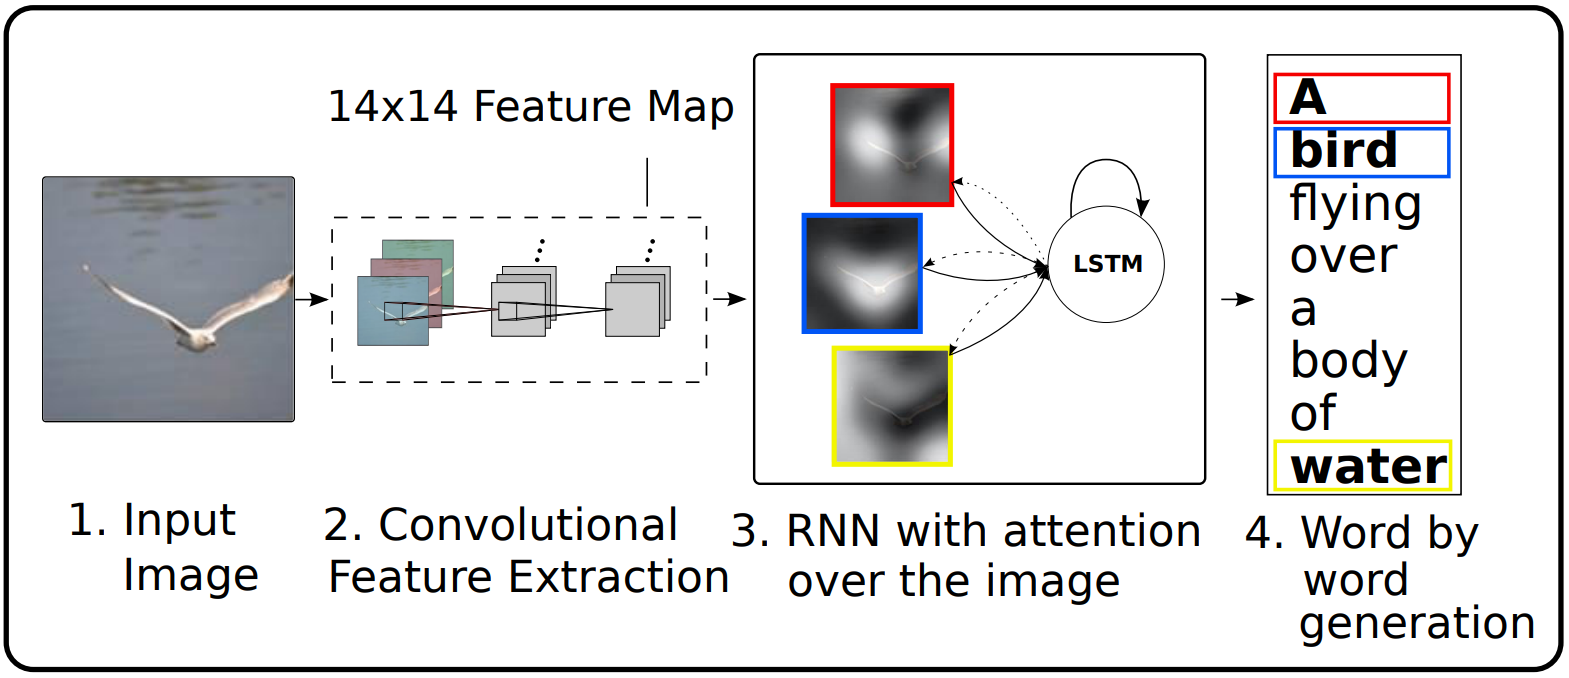
\includegraphics[width=0.7\linewidth]{./img/img_captioning.png}
\caption{
    Diagram of natural language image description using Attention
    (from \cite{ref:img-captioning}).
}
\label{fig:description}
\end{center}
\end{figure}

\subsection{Motivation and Objectives}
In spite of the recent adoption of Attention by a variety of Deep Learning models
and the significant improvements it has shown, we conjecture that there are still many other tasks
that are still not explored.
Current works also tend to focus more on the filtering functionality of Attention,
but there are other aspects
-- such as the allocation of mental resources over time -- that can be of potential benefit
(we further discuss the taxonomy of Attention in following sections).
Furthermore, we note that Attention models currently being used
are very specific to each problem in question.
Some works propose a higher level of generalization~\cite{ref:rec-models},
but we believe it is possible to go further.
Therefore, the specific objectives of this work are:
\begin{itemize}
    \item To perform an extensive literature review on the use of Attention
        in modern Deep Learning;
    \item From the perspective of a theoretical framework of Attention (from areas such as psychology and neuroscience),
        identify in the current literature opportunities in the form of theoretical aspects to be explored that are of
        potential benefit for the area;
    \item To identify a specific problem
        (in robotics, vision, natural language or other area) with
        improvement potential through the use of Attention, proposing and implementing
        a solution based on the findings of the work to
        validate the ideas and evaluate them in an application.
    %\item To study the viability of generalization of Attention
    %    to broader areas in AI other than Deep Learning.
\end{itemize}

The main contribution of the work proposed we wish to accomplish is to
\emph{establish a theoretical framework of Attention as a series of components
    and its applicabilities to Deep Learning.}
Recent works show that the effort on establishing more general concepts and frameworks for
Deep Learning design has been broadly useful.
Examples include the ideas of \emph{Curriculum Learning}~\cite{ref:curriculum}
and \emph{Generative Adversarial Networks}~\cite{ref:gans}.

\section{Activities}
\label{sec:activities}
The work can be summarized in three main activities (or \textbf{phases}):
\begin{itemize}
    \item \textbf{1. Literature Review}: an extensive survey on current uses of Attention in modern
        Deep Learning.
    \item \textbf{2. Proposal of an Attention framework for Deep Learning}: \
        defining a component set of Attention elements currently used in Deep Learning design from results of the previous phase and further survey.
    \item \textbf{3. Implementation and validation of Attention in Deep Learning}:
        proposing a model with components of Attention and evaluating it on a set of tasks.
\end{itemize}

More specifically, the activities to be executed are:

\begin{itemize}
    \item \textbf{A1.1 - Theoretical definition of Attention and its components:}
        From a variety of previous works~\cite{ref:helgason}\cite{ref:esther-thesis},
        we establish a theoretical framework of Attention
        on which all later work will be based.
        It is worth noting that this theoretical framework is not necessarily the same as the framework
        we propose to produce specifically for Deep Learning in phase 2. It will work as the base that will be used to organize and classify the current literature.

    \item \textbf{A1.2 - Elaboration of survey:}
        Exploration of selected work under the point of view of the theoretical framework established
        in \textbf{A1.1}.
        For each work, we identify the main components of Attention the authors use, the consequences for the
        performance in the application domain and elaborate a critical evaluation.

    \item \textbf{A2.1 - Establishment of Attention components for specific Deep Learning domains:}
        From the theoretical framework obtained in \textbf{A1.1}
        and the exploration of current uses and results in \textbf{A1.2},
        we devise sets of useful components of Attention for specific main problem domains
        in which Deep Learning is broadly used,
        such as image classification, text-to-speech, language translation, image segmentation.

    \item \textbf{A2.2 - Establishment of Attention framework for Deep Learning:}
        From the theoretical framework obtained in \textbf{A1.1},
        exploration of current uses and results in \textbf{A1.2} and
        results from \textbf{A2.1},
        we elaborate a set of components of Attention under a single framework to be applied to more
        general areas of use of Deep Learning,
        such as Computer Vision, Sequence Processing, Program Composition.

    \item \textbf{A3.1 - Arrangement of experiments:}
        From the framework obtained in phase 2, we select a set of problem domains (such as text-to-speech),
        Deep Learning models to use, components of Attention to implement and metrics to evaluate the task.
        The activity aims at selecting all main devised components from phase $2$ in order
        to evaluate the real consequences of their adoption against what was predicted.

    \item \textbf{A3.2 - Execution of experiments:}
        We implement and execute the planned experiments following a pre-defined protocol that
        pays particular attention to reproducibility.

    \item \textbf{A3.3 - Evaluation of experimental results:}
        We evaluate the results using established metrics for each experiment,
        elaborating discussions that include exciting aspects of the results in general and
        comparisons between the theoretical predictions and tangible outcomes.
        It is worth noting that the metrics we'll use will vary depending on the specific problem,
        but they will always be selected to reflect the improvement of the models with the use of
        attention.
\end{itemize}

\section{Use of results}
The findings of the work may be of benefit for the Deep Learning community.
On a previous and related work~\cite{ref:erik-esther}, the authors built a fully convolutional network
for the prediction of visual saliency maps, achieving top-10 results in a variety of metrics
on the MIT300 benchmark. The results of the work (model weights/code) were made available to the public.
In a similar fashion, we intend to make all findings public, as well as make the data/code obtained openly
available -- along with documentation and tutorials.

%\renewcommand\bibname{References\vspace*{10mm}}
\printbibliography

%\begingroup
%\let\clearpage\relax
%\bibliographystyle{plain}
%\bibliography{proposal.bib}
%\printbibliography
%\endgroup

\end{document}
